\documentclass[10pt,a4paper]{article}

\usepackage[utf8]{inputenc}		% Configuro la codificación
\input{.command.tex}
% En el siguiente archivo se configuran las variables del trabajo práctico
%% \providecommand es similar a \newcommnad, salvo que el primero ante un 
%% conflicto en la compilación, es ignorado.

% Al comienzo de un TP se debe modificar los argumentos de los comandos

\providecommand{\myTitle}{ACTIVIDAD 3}
\providecommand{\mySubtitle}{Fuentes conmutadas}

\providecommand{\mySubject}{Diseño de Circuitos Electrónicos (86.10)}
\providecommand{\myKeywords}{UBA, Ingeniería, C2}

\providecommand{\myAuthorSurname}{Alonso, Manso, Zuccolo}
\providecommand{\myTimePeriod}{Año 2018 - 2\textsuperscript{do} Cuatrimestre}

% No es necesario modificar este %%%%%%%%%%%%%%
\providecommand{\myHeaderLogo}{header_fiuba}
%%%%%%%%%%%%%%%%%%%%%%%%%%%%%%%%%%%%%%%%%%%%%%%%

% Si se utilizan listings, definir el lenguaje aquí
\providecommand{\myLanguage}{matlab}

% Crear los integrantes del TP con el comando \PutMember donde
%%		1) Apellido, Nombre
%%		2) Número de Padrón
%%		3) E-Mail
\providecommand{\MembersOnCover}[0]
{		
		\PutMember{Alonso, Gustavo Gabriel} {96119} {gustavoalon19@gmail.com}
		\PutMember{Manso, Juan} {96133} {juanmanso@gmail.com}
		\PutMember{Russo, Nicolas Emanuel} {93211} {nicolasrusso291@gmail.com}
		\PutMember{Zuccolo, Florencia} {96628} {florenciaz618@gmail.com}
}

\providecommand{\myGroupNumber}{10}

\Pagebreaktrue		% Setea si hay un salto de página en la carátula
\Indextrue
\Siunitxtrue			% Si quiero utilizar el paquete, \siunixtrue. Si no \siunixfalse
\Todonotestrue		% Habilita/Deshabilita las To-Do Notes y las funciones \unsure, \change, \info, \improvement y \thiswillnotshow.
\Listingsfalse
\Keywordsfalse
\Putgrouptrue		% Habilita/Deshabilita el \myGroup en los headers
\Videofalse
				% Archivo con los comandos globales como Título y autores
%Preambulo para articulo científico de LaTeX

\usepackage[a4paper,left=3cm,right=3cm,bottom=3.5cm,top=3.5cm]{geometry} 	% Configuro la geometría del papel
%\usepackage{microtype}								% Mejora el "spacing" de las palabras
\usepackage[spanish]{babel} 							% Compatibilizo los signos del español
	\addto\captionsspanish{\renewcommand{\tablename}{Tabla}}		%% Redefino nombres preestablecidos por Babel
	\addto\captionsspanish{\renewcommand{\listtablename}{Índice de tablas}}	%% y así en vez de Cuadro dirá Tabla.
\usepackage{amsmath, amsfonts, amssymb}						% Entornos matemáticos, fuentes y símbolos
\usepackage{graphicx}								% Necesario para insertar figuras
\usepackage{fancyhdr}								% Para manipular headers y footers
\usepackage[usenames,dvipsnames]{color}						% \color{color deseado} {lo que querés que tenga color}
\usepackage{subcaption}								% Permite captions del tipo 1a, 1b
\usepackage{multirow}								% Para tablas
%\usepackage{slashbox}								% Cuadro divido en tablas
\usepackage{diagbox}
\usepackage{float}
\usepackage{multicol}

% Para video
\ifVideo
	\usepackage{media9}
	\addmediapath{./../reportes/}
\fi

%\usepackage{times}
%\usepackage{mathtools}
%\usepackage{upgreek} % letras griegas sin cursiva
%\usepackage{cancel}
\usepackage{rotating}
\usepackage{tikz}
\usepackage{pgfplots}
%	\pgfplotsset{compat=1.12}
	\usetikzlibrary{plotmarks}% matlab2tikz
\usepackage{grffile}% matlab2tikz 
	\usetikzlibrary{calc,patterns,decorations.pathmorphing,decorations.markings}

\ifListings
	\usepackage{listings}

	\providecommand{\lstinputpath}[1]{\lstset{inputpath=#1}}

%	\input{.lst_default.tex}
	\input{.lst_matlab.tex}
%	\input{.lst_c.tex}
%	\input{.lst_c++.tex}
	
% 	\input{.lst_pseudocode.tex}


\fi

\ifSiunitx
\usepackage{siunitx}											% Unidades: \SI {cantidad} {\unidad} (necesita texlive-science)
	\sisetup{load-configurations = abbreviations}							% Habilita poner \cm en vez de \centi\metre
	\sisetup{output-decimal-marker = {,}}									% Cambia los puntos decimales por comas
	\sisetup{per-mode = fraction}											% Pone las unidades como fracción
	\sisetup{quotient-mode = fraction}										
\fi


\ifTodonotes
\usepackage{xargs}
\usepackage[colorinlistoftodos,prependcaption,textsize=tiny]{todonotes}


	\newcommandx{\Juan}[2][1=]{\todo[linecolor=red,backgroundcolor=red!25,bordercolor=red,#1]{#2}}
	\newcommandx{\Flor}[2][1=]{\todo[linecolor=blue,backgroundcolor=blue!25,bordercolor=blue,#1]{#2}}
	\newcommandx{\Gus}[2][1=]{\todo[linecolor=green,backgroundcolor=green!25,bordercolor=green,#1]{#2}} % OliveGreen
	\newcommandx{\Nico}[2][1=]{\todo[linecolor=yellow,backgroundcolor=yellow!25,bordercolor=yellow,#1]{#2}}
	\newcommandx{\thiswillnotshow}[2][1=]{\todo[disable,#1]{#2}}
\fi


\usepackage{booktabs}														% Permite hacer tablas sin separadores en el medio
\usepackage{placeins}														
		\let\Oldsection\section												%% Permite que los flotantes (como figuras) no aparescan
	\renewcommand{\section}{\FloatBarrier\Oldsection}						%% antes o después de su sección correspondiente.
		\let\Oldsubsection\subsection
	\renewcommand{\subsection}{\FloatBarrier\Oldsubsection}		
		\let\Oldsubsubsection\subsubsection
	\renewcommand{\subsubsection}{\FloatBarrier\Oldsubsubsection}
\usepackage{hyperref}														% Debe ser agregado al final del preambulo

\hypersetup
{    bookmarks=true,         % show bookmarks bar?
     unicode=false,          % non-Latin characters in Acrobat’s bookmarks
     pdftoolbar=true,        % show Acrobat’s toolbar?
     pdfmenubar=true,        % show Acrobat’s menu?
     pdffitwindow=false,     % window fit to page when opened
     pdftitle={\myTitle},    		 % title
     pdfauthor={\myAuthorSurname},   % author
	 pdfcreator={\myAuthorSurname},	 % creator = author
     pdfsubject={\mySubject},		 % subject of the document
     pdfkeywords={\myKeywords},
     colorlinks=true,        % false: boxed links; true: colored links
     linkcolor=black,        % color of internal links (change box color with linkbordercolor)
     citecolor=black,        % color of links to bibliography
     filecolor=magenta,      % color of file links
     urlcolor=cyan           % color of external links
}

%Configuro la pagina con los encabezaos y pies de paginas
\pagestyle{fancy}										% Para agregar encabezados y pie de paginas	
%\lhead{\mySubject}										% Encabezado izquierdo
\lhead{DCE (86.10)}
\rhead{\includegraphics[scale=0.15]{\myHeaderLogo}} 	% Encabezado derecho (logo de la FIUBA)	
\ifPutgroup
\chead{\texttt{Grupo Nº\myGroupNumber} \\ \textit{\footnotesize{\myTimePeriod}}}
\fi				

%% Este archivo contiene las funciones auxiliares para escribir en LaTeX
%% Dichas funciones resuelven la sintaxis de generar figuras, por ejemplo,
%% dejando el código más compacto y facilitando la corrección del mismo.



% Comando para graficar eps. 1er arg, escala. 2do, ruta. 3ro, caption. 4to, label.
\providecommand{\HgraficarEPS}[4]{
			\begin{figure}[h!]
				\centering
					\scalebox{#1}{\input{#2}}
					\caption{#3}
					\label{#4}
			\end{figure}

}

\providecommand{\HgraficarPNG}[4]{
			\begin{figure}[h!]
				\centering
					\includegraphics[scale=#1]{#2}
					\caption{#3}
					\label{#4}
			\end{figure}

}


% Comando para graficar eps en el lugar previsto.
\providecommand{\graficarEPS}[4]{
			\begin{figure}[h]
				\centering
					\scalebox{#1}{\input{#2}}
					\caption{#3}
					\label{#4}
			\end{figure}

}

\providecommand{\graficarPNG}[4]{
			\begin{figure}[h]
				\centering
					\includegraphics[scale=#1]{#2}
					\caption{#3}
					\label{#4}
			\end{figure}

}

\providecommand{\underuparrow}[2]{\underset{\underset{#2} \uparrow} #1 }

\providecommand{\cltext}[2]{\color{#1}{\huge{#2}}}
\providecommand{\cstext}[2]{\color{#1}{\large{#2}}}

\providecommand{\lsi}[1]{\large\si{#1}}
\providecommand{\lsio}[0]{\large\si{\ohm}}
\providecommand{\lsiv}[0]{\large\si{\volt}}
\providecommand{\lsia}[0]{\large\si{\ampere}}
\providecommand{\lSI}[2]{\large\SI{#1}{#2}}


		% Se proveen un conjunto de funciones extras

% Defino el path de los includegraphics
\graphicspath{{./Figuras/}}		% Directorio que contiene los graficos

% Defino el path para los input de .tex y de .eps
\makeatletter
\def\input@path{{./Figuras/}{./Secciones/}{./Cover_page/}{../Octave/graficos/}}
\makeatother

% Defino el path del listings
\ifListings
%% Cambiar el nombre de la carpeta si se utilizan Listings
	\lstinputpath{{../Octave/}}
\fi

\definecolor{myred}{rgb}{0.5,0,0}
\definecolor{mygreen}{rgb}{0,0.5,0}



\begin{document}
		% Carátula (formal o simple,_formal o _simple respectivamente) con Resumen
		% incluido e Índice (si es necesario configurar en config.tex) del informe
		\begin{titlepage}
	
		\thispagestyle{empty}

		\begin{center}
			
\includegraphics[scale=0.3]{fiuba}\\
			\large{\textsc{Universidad de Buenos Aires}}\\
			\large{\textsc{Facultad De Ingeniería}}\\
			\small{\myTimePeriod}
		\end{center}

		\vfill

		\begin{center}
			\Large{\underline{\textsc{\mySubject}}}
		\end{center}

		\vfill

		\begin{tabbing}
			\hspace{2cm}\=\+\myTitle\\
				TEMA: \mySubtitle\\
				FECHA: \today\\
				\ifPutgroup
				GRUPO: \texttt{\myGroupNumber}\\
				\fi

			\\
				\MembersHeader
				\MembersOnCover	
		\end{tabbing}

		\begin{abstract}
			\input{0_resumen.tex}
		\end{abstract}

	\ifKeywords
		\begin{center}
			\emph{Palabras Clave: \myKeywords}
		\end{center}
	\fi	

		\vfill
	
\end{titlepage}

\ifPagebreak
	\thispagestyle{empty}
	\ifIndex
		\tableofcontents
%		\listoffigures
%		\listoftables
	\fi

	\pagebreak
\fi


	\setcounter{page}{1}

		%\section{Polarización}\label{sec:pol}
			\begin{quote} \textit{1) Estudiar las corrientes y tensiones en todos los componentes en función del tiempo, desde que se enciende el regulador ($t=0$) hasta régimen permanente. En particular, en régimen permanente, estudiar en detalle las corrientes y tensiones en un intervalo de unos pocos periodos.}
\end{quote}

%\HgraficarPNG{0.4}{fly}{Regulador \textit{Flyback} aislado.}{fig:cto}

\begin{figure}[H]
	\centering
	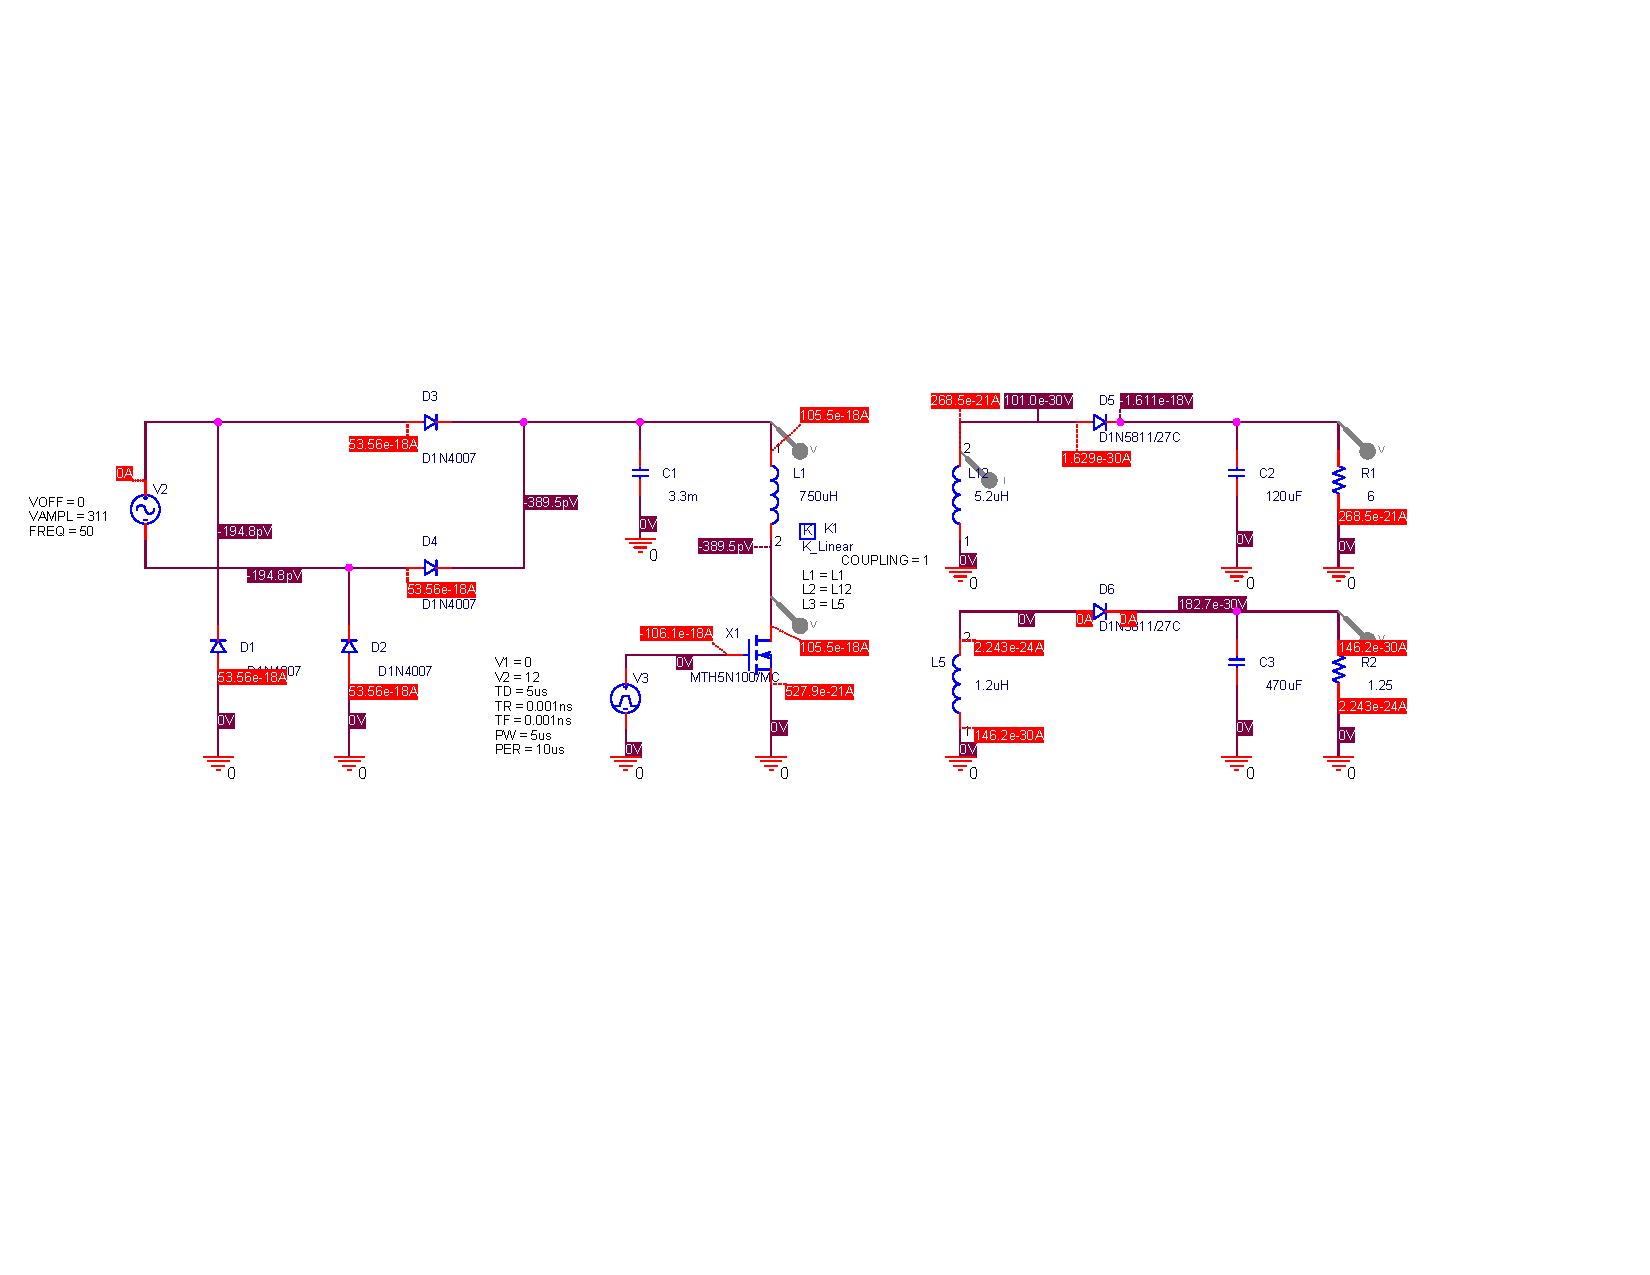
\includegraphics[scale=0.5]{Figuras/1_esquematico.pdf}
	\caption{Circuito bajo análisis con \textit{PSpice}.}
	\label{fig:esq}
\end{figure}


\Flor{Simulación hecha con $Vimax = \sqrt{2} 220V = 311V. }
\begin{figure}[H]
	\centering
	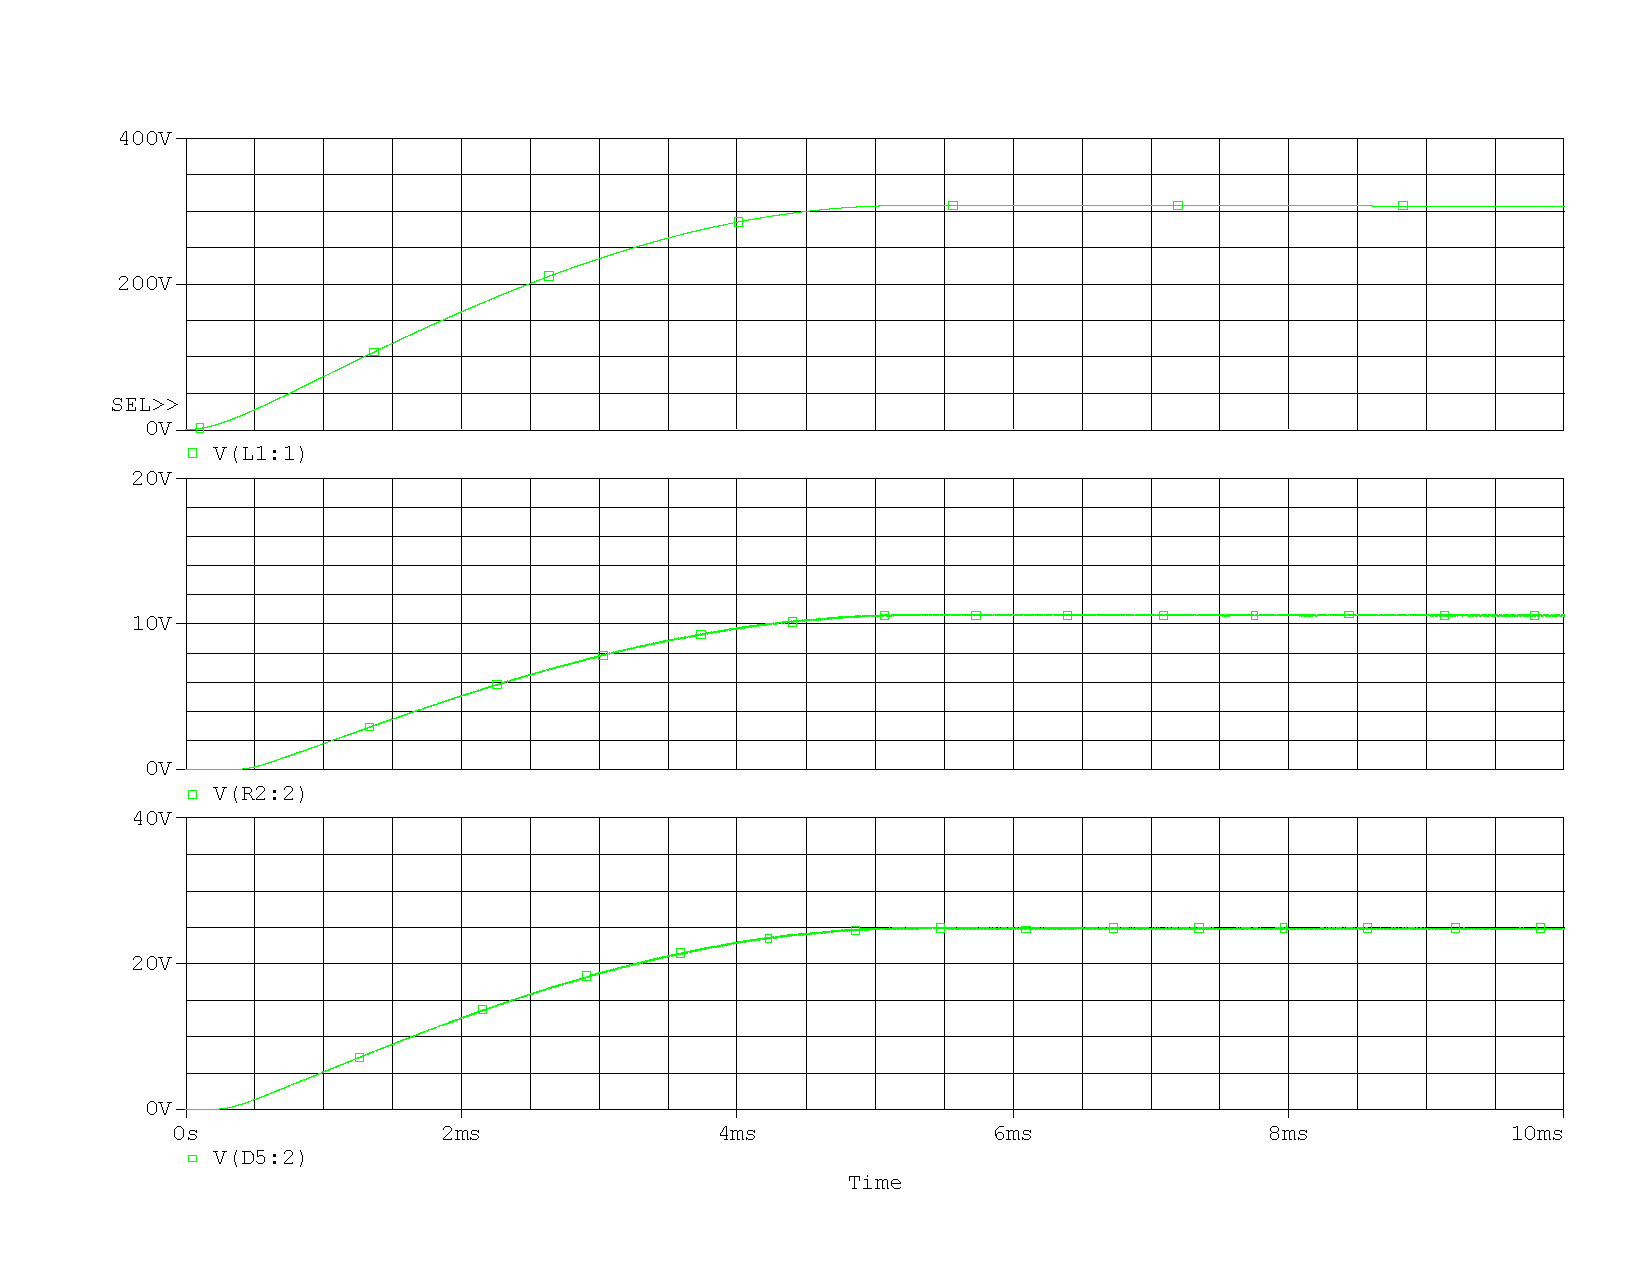
\includegraphics[scale=0.5]{Figuras/1_transitorio_con_rectificador.pdf}
	\caption{Transitorio.}
	\label{fig:transitorio}
\end{figure}

\begin{figure}[H]
	\centering
	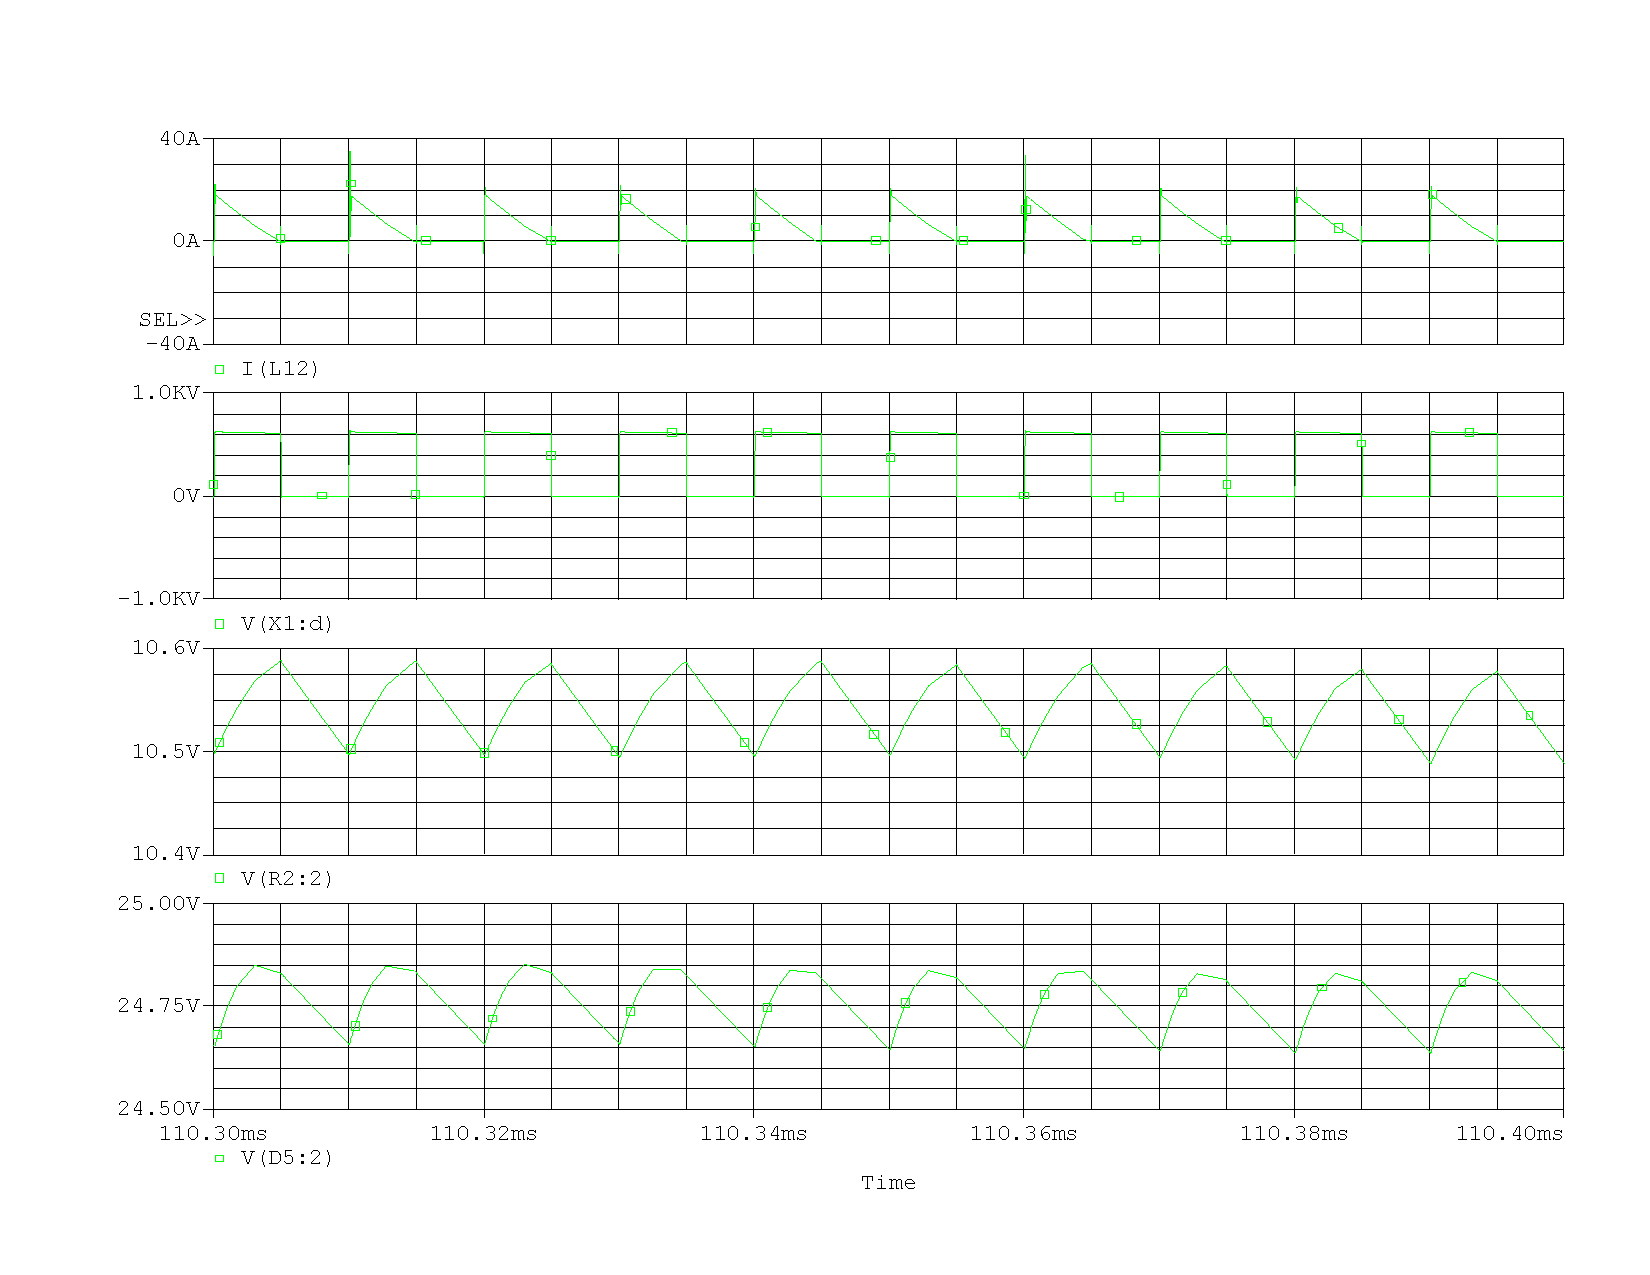
\includegraphics[scale=0.5]{Figuras/1_regimen_permanente.pdf}
	\caption{Régimen permanente.}
	\label{fig:permanente}
\end{figure}



		%\section{Variación de la carga}\label{sec:variacion_carga}
			%\begin{quote} \textit{2) Luego de haber estudiado como está operando el circuito con las cargas $R_1$ y $R_2$ en su valor de diseño (\SI{6}{\ohm} y\SI{1.25}{\ohm} respectivamente), estudiar cómo opera el circuito si éstas varían hacia valores mayores y menores.}
%\end{quote}
Luego, se analizó el comportamiento del circuito ante variaciones de carga, obteniéndose \ref{fig:var_R1} y \ref{fig:var_R2}.

\begin{figure}[H]
	\centering
	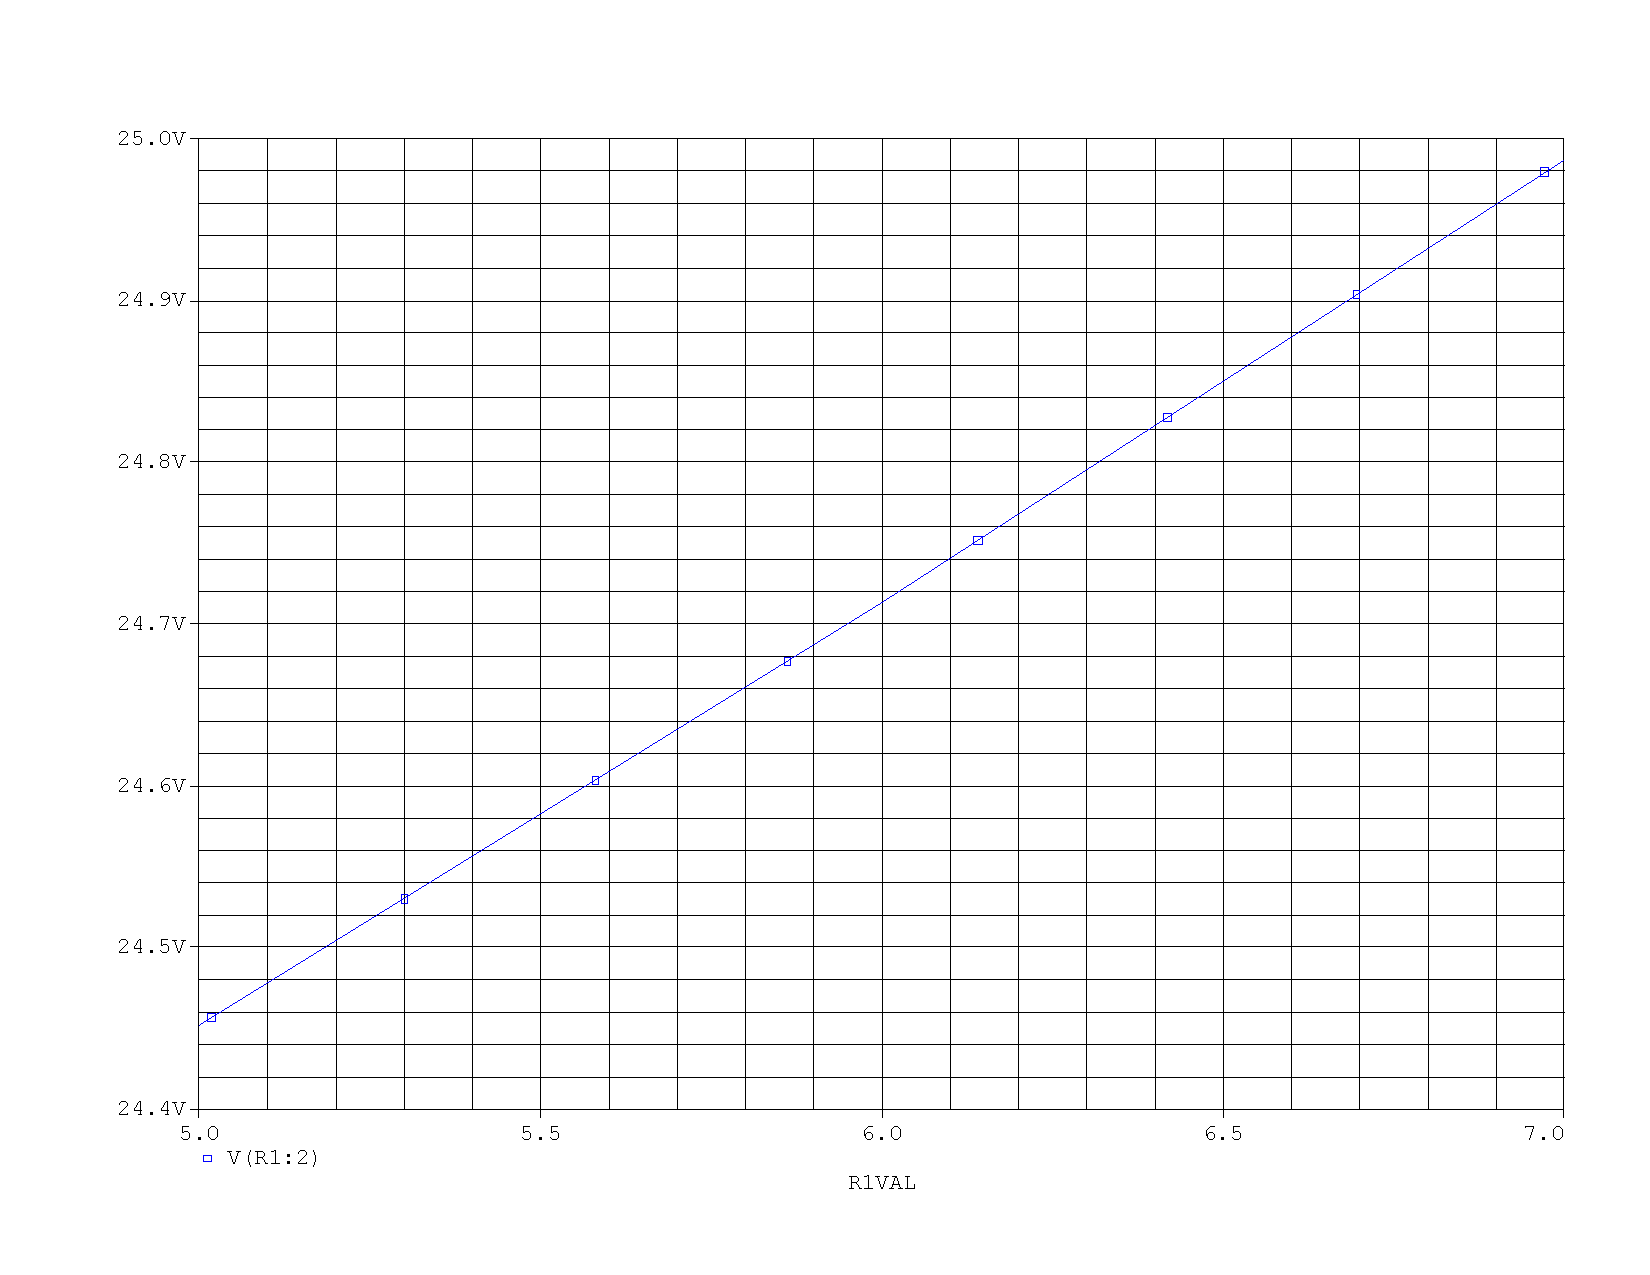
\includegraphics[scale=0.5]{Figuras/2_var_R1.pdf}
	\caption{Variación de $R_1$.}
	\label{fig:var_R1}
\end{figure}


%\begin{figure}[H]
%	\centering
%	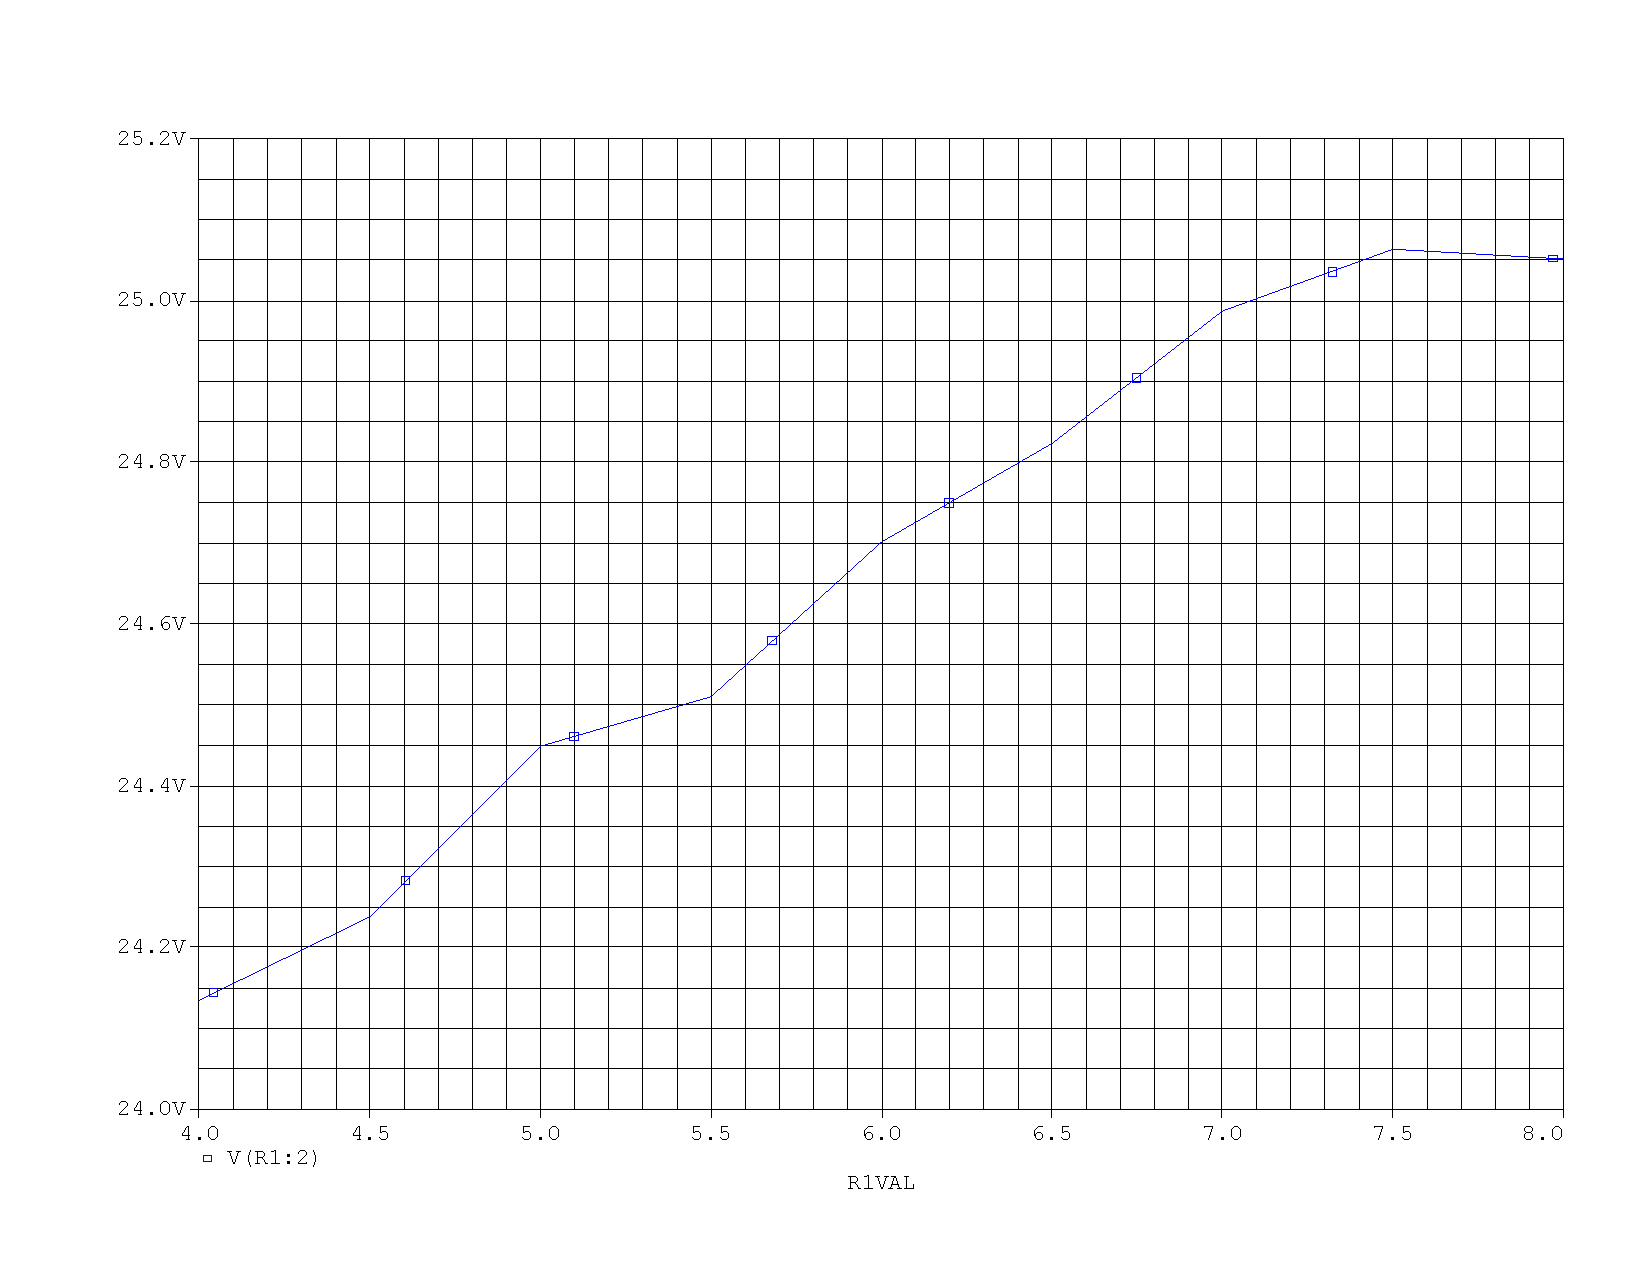
\includegraphics[scale=0.5]{Figuras/2_var_R1_v2.pdf}
%	\caption{Variación de $R_1$.}
%	\label{fig:var_R1}
%\end{figure}


\begin{figure}[H]
	\centering
	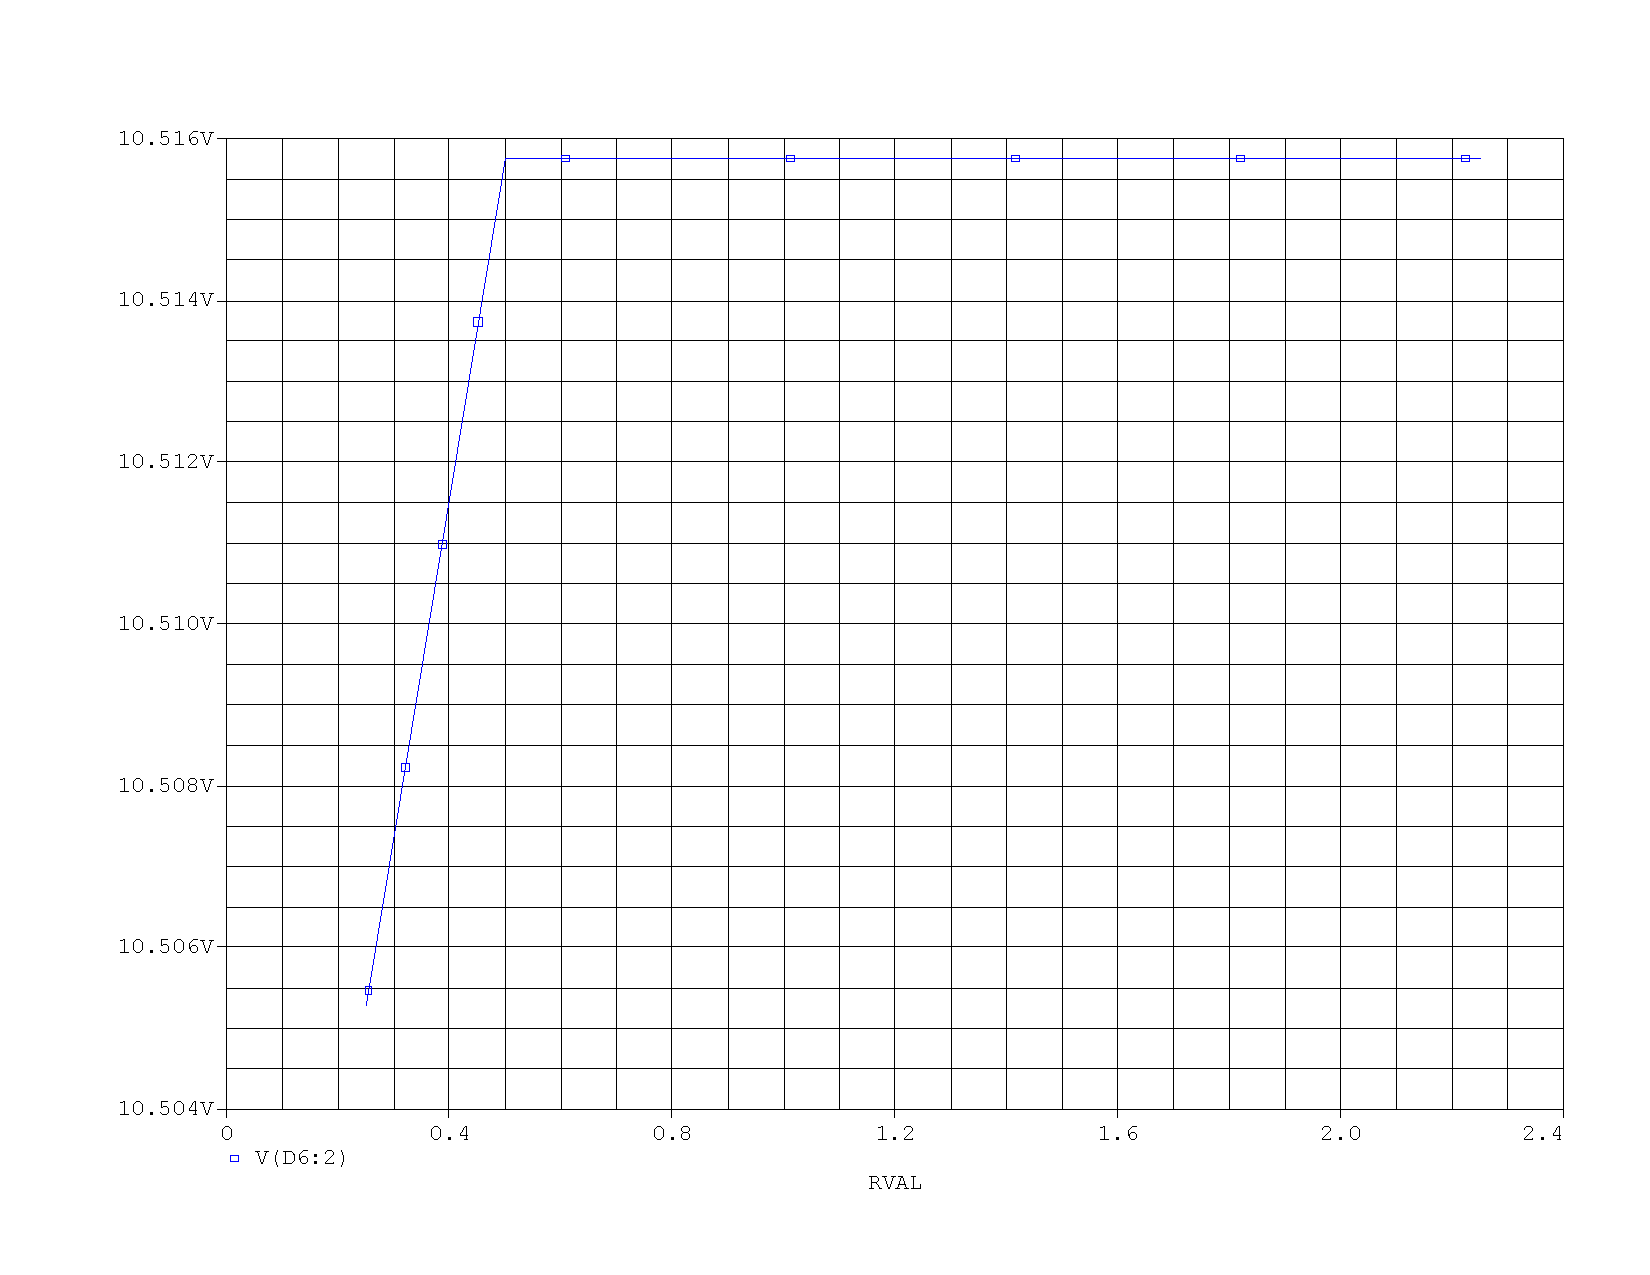
\includegraphics[scale=0.5]{Figuras/2_var_R2.pdf}
	\caption{Variación de $R_2$.}
	\label{fig:var_R2}
\end{figure}




		%\section{Estudio de componentes}\label{sec:componentes}
			\begin{quote} \textit{3) En base al estudio del ítem anterior verificar si los semiconductores sobrevivirán el estrés del régimen transitorio y la operación en régimen permanente. O sea, determinar si los semiconductores $M_1$, $D_1$ a $D_7$ son adecuados para este diseño, justificar y en caso de que alguno o algunos no lo sean, encontrar un sustituto que sí. Justificar este estudio en las características publicadas por los fabricantes de los semiconductores. }
\end{quote}

		%\section{Variación del ciclo de trabajo}\label{sec:duty_cycle}
			\begin{quote} \textit{ 4) El regulador se ha diseñado para operar en modo discontinuo con $D<0,5$. Verificar si para $D>0,5$ el regulador pasa a operar en modo continuo. ¿Qué observará en las señales de tensión y corriente de todos o alguno de los componentes para determinar el si el regulador está operando en modo continuo o discontinuo?}
\end{quote}

		%\section{Valor del capacitor}\label{sec:C3}
			\begin{quote} \textit{5) Determinar el valor adecuado de C3.}
\end{quote}

		%\section{Características de capacitores}\label{sec:caps}
			\begin{quote} \textit{6) Dimensionar todos los capacitores, o sea, tamaño, formato, tecnología, tolerancia, máxima potencia y/o tensión y temperatura, resistencia efectiva serie, frecuencia de operación máxima, tiempo de vida útil, etc.}
\end{quote}
\Flor{Creo que 120uF y 470uF vienen solo electroliticos, aunque son malos para alta frecuencia}
\begin{table}[H]
	\centering
	\begin{tabular}{cccccccc}
		\toprule
		& Valor & $V_{max}$ & Tipo & ESR & tol. & vida útil &f \\
		\midrule
		$C_1$ & \SI{470}{\micro\farad} & \SI{25}{\volt} & electrolítico &  & 10\% & &  \\
		$C_2$ &\SI{120}{\micro\farad} & \SI{16}{\volt} & electrolítico & & 10\% & &\\
		$C$ &\SI{3300}{\micro\farad} & \SI{250}{\volt} & electrolítico & \SI{0.4}{\ohm} & 20\% &  2000hs a \SI{105}{\celsius} & \\
		\bottomrule
	\end{tabular}
\end{table}

		%\section{Controlador}\label{sec:controlador}
			\begin{quote} \textit{7) Se requiere que el regulador actúe en forma automática ante cambios en la carga y/o en la fuente de entrada, para lo cual es necesario diseñar un circuito controlador que sense la tensión de salida y varíe apropiadamente el ciclo de servicio D (reemplazando el generador de pulsos mostrado en el esquema presentado en esta actividad). Esto puede lograrse con un circuito auotoscilante (generalmente discreto con unos pocos transistores) o con un circuito integrado dedicado. Investigar ambas soluciones y plantear una adecuada.}
\end{quote}

\Flor{TL494}

		%\section{Protección}
			\begin{quote} \textit{8) Considerar también la forma de proteger la carga, el regulador y la fuente primaria implementando los circuitos adecuados. Este último tema no es obligatorio para la presente actividad y puede omitirse. Sin embargo se recomienda tenerlo presente en todo diseño de reguladores conmutados o lineales.}
\end{quote}


		%\section{Conclusiones}\label{sec:conclusiones}
			\input{9_conclusiones.tex}
	% \appendix
\end{document}
